\documentclass[12pt,a4paper,final]{article}
\usepackage[left=2.5cm,right=2.5cm,top=2.5cm,bottom=2.5cm]{geometry}

%% IDIOMA
\usepackage[utf8]{inputenc}
\usepackage[portuguese]{babel}

%% TRANSFORMAÇÕES ESTILO CSS
\usepackage{graphicx}

%% ESTÉTICA
\usepackage{enumerate}
\usepackage{booktabs}
\usepackage{amsmath, amsthm, amssymb, amsfonts}
\usepackage{multirow}
\usepackage[hyphens]{url}
\usepackage{subfig}

%% FONTE
\usepackage[T1]{fontenc}
%\usepackage[sc]{mathpazo} % Palatino with smallcaps
\usepackage{mathptmx}
\usepackage{eulervm} % Euler math

%% TIPOGRAFIA
\usepackage{parskip}
\usepackage[activate={true,nocompatibility},final,tracking=true,kerning=true,spacing=true,factor=1100,stretch=10,shrink=10]{microtype}

%% CODIGO
\usepackage{listings}
\usepackage{color}

\definecolor{dkgreen}{rgb}{0,0.6,0}
\definecolor{gray}{rgb}{0.5,0.5,0.5}
\definecolor{mauve}{rgb}{0.58,0,0.82}

\lstset{frame=tb,
  aboveskip=3mm,
  belowskip=3mm,
  showstringspaces=false,
  columns=flexible,
  basicstyle={\small\ttfamily},
  numbers=none,
  numberstyle=\tiny\color{gray},
  keywordstyle=\color{blue},
  commentstyle=\color{dkgreen},
  stringstyle=\color{mauve},
  breaklines=true,
  breakatwhitespace=true,
  tabsize=3
}

\title{Relatório 6 de TCC2/IC}
\author{Ly Sandro Amorim de Campos Salles\\Departamento de Física\\Universidade Federal do Paraná}
\date{\today}

\begin{document}
	\maketitle

  Desde o último encontro foram realizadas as seguintes atividades:

  A finalização do novo programa de simulações de autômatos celulares, disponível, com histórico de modificações, no endereço \url{https://github.com/Ly54ndr0/CellularAutomataExplorer}.

  Foi verificado que os algoritmos utilizados estão corretos e retornam valores corretos.

  Obtenção de cinco conjunto de dados, com 20000 pontos cada, para cada combinação de $q$ e $L$ com $q\in\{$ 
  $0.1,$ $0.2,$ $0.3,$ $0.4,$ $0.5,$ $0.6,$ $0.7,$ $0.8,$ $0.9,$
  $1,$ $1.2,$ $1.4,$ $1.6,$ $1.8,$ 
  $2,$ $2.2,$ $2.4,$ $2.6,$ $2.8,$ 
  $3,$ $3.2,$ $3.4,$ $3.6,$ $3.8,$
  $4,$ $4.2,$ $4.4,$ $4.6,$ $4.8,$
  $5,$ $5.2,$ $5.4,$ $5.6,$ $5.8,$
  $6,$ $6.2,$ $6.4,$ $6.6,$ $6.8,$
  $7,$ $7.2,$ $7.4,$ $7.6,$ $7.8,$
  $8,$ $8.2,$ $8.4,$ $8.6,$ $8.8,$
  $9,$ $9.2,$ $9.4,$ $9.6,$ $9.8,$ $10,$
  $11,$ $12,$ $13,$ $14,$ $15,$ $16,$ $17,$ $18,$ $19,$ $20,$
  $22,$ $24,$ $26,$ $28,$ $30,$ $32,$ $34,$ $36,$ $38,$ $40,$
  $42,$ $44,$ $46,$ $48,$ $50,$ $52,$ $54,$ $56,$ $58,$ $60,$
  $65,$ $70,$ $75,$ $80,$ $85,$ $90,$ $95,$ $100,$ $110,$
  $120,$ $130,$ $140,$ $150,$ $160,$ $170,$ $180,$ $190,$
  $200,$ $220,$ $240,$ $260,$ $280,$ $300,$ $320,$ $340,$ $360,$ $380,$
  $400,$ $420,$ $440,$ $460,$ $480,$ $500,$ $520,$ $540,$ $560,$ $580,$
  $600,$ $620,$ $640,$ $660,$ $680,$ $700,$ $720,$ $740,$ $760,$ $780,$
  $800,$ $820,$ $840,$ $860,$ $880,$ $900,$ $920,$ $940,$ $960,$ $980,$
  $1000\}$ e $L\in \{50, 100, 250, 500, 1000, 2000\}$.

  Foi verificado que não ocorre a sopreposição da curva do potencial de Lennard-Jones no gráfico de afinidade em função de $q$, como ilustrado nas Figuras ??.

  %\begin{figure}
  %  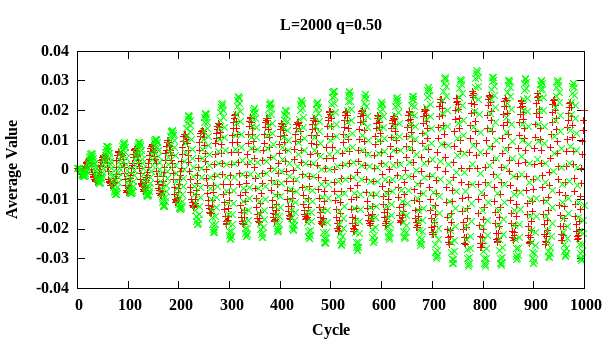
\includegraphics[width=\linewidth]{dataL2000Q50AvgStateThresVScycle.png}
  %  \caption{L = 50}
  %  \label{fig:}
  %\end{figure}

  Foi lido o ``Material de Estudos da Certificação CPA-10: Volume 4, Princípios de Investimento'', da Associação Brasileira das Entidades dos Mercados Financeiro e de Capitais (ANBIMA), o qual, entre outros assuntos, inclui a descrição de liquidez.
  
  Foi escrito o seguinte protótipo de resumo:\\
  \textit{Utilizando um autômato celular bidimensional para simulações de compra e venda de agentes em um mercado, determinamos a intensidade com que esses agentes tendem a tomar decisões em conjunto, denominada afinidade, em função da liquidez do mercado. Essas simulações foram feitas para vários números diferentes de agentes. Descobrimos, nessa análise positiva, que a afinidade é uma função sigmóide da liquidez do mercado, variando um pouco com o número de agentes nesse mercado.}

  Para os próximos dias, estas serão as tarefas realizadas:
	\begin{enumerate}
		\item Leitura do artigo ``Stochastic Cellular Automata Model for Stock Market Dynamics'' dos autores M. Bartolozzi e A. W. Thomas;
		\item Pesquisa sobre como a volatilidade de mercado influencia na aglomeração dos agentes;
	\end{enumerate}

\end{document}
